\documentclass[12pt,twocolumn]{article}
\usepackage{graphicx}
\usepackage{float}
%\usepackage{wrapfig}
\setlength{\textwidth}{6.5in}
\setlength{\textheight}{9.9in}
\setlength{\oddsidemargin}{0.0in}
\setlength{\evensidemargin}{0.0in}
\setlength{\topmargin}{-2.5 cm}
\setlength{\parskip}{0.7\baselineskip} % space between paragraphs
\setlength{\parindent}{0 cm} % increase this if you like paragraphs to be indented
\usepackage{hyperref}
\usepackage{xcolor}
\usepackage{natbib}  % For bibliography styles

\pagestyle{empty}

\newcommand{\e}{\mathrm{e}}

\begin{document}

\title{\bf{Constructing a Pendulum to Determine its Period and
Q Factor}}
\author{Adam Omarali}
\date{December 6 2023 \linebreak
\textcolor{red}{All sections in red are copied.} \bf{Black is all new content.}
}
\maketitle

\section{Introduction}

\textcolor{red}{By designing a two string pendulum attached
to a yellow ball with a variable length, a given
model is tested against empirical results to
better inform the accuracy of the model.}

\textcolor{red}{The initial angle versus period, amplitude
over time, length versus period and length
versus Q Factor are analyzed with the aid of
video tracking software Tracker[1].}

\subsection*{Equations}

A power function describes the relationship between pendulum length ($L$) and period $T$.

\begin{equation}
    \label{Emp_Period}
    T = p L^q
\end{equation}

The range of parameters $p = 1.98 \pm 0.01 m^{-1}s$ and
$q = 0.474 \pm 0.007$ are empirically found to fall slightly outside the 
expected values of $p = 2$ and $q=0.5$ given by [2].

A pendulum's initial angle release is found to have an even powered quadratic relationship with its period.

\begin{equation}
    \label{Period_Angle}
    T = T_0 (1 + B\theta + A\theta^2)
\end{equation}

The odd power term B is found to be experimentally zero, while $T_0 = 1.337 \pm 0.001 s$,
and, $A = 0.043 \pm 0.001 rad^{-2}$. No asymmetry is found.
Amplitude and period are not found to be independent 
unless the small angle range of $-0.5 \leq \theta \leq 0.5 rad$.

The damped harmonic oscillator (Equation \ref{DampedHarmonic}) accurately gives the
angle over time ($\pm 0.02rad$) provided an initial
angle ($\theta_0$), the time ($t$), the decay constant
($\tau$), the period (T) and a time offset ($\phi$).

\begin{equation} 
    \label{DampedHarmonic}
    \theta(t) = \theta_0 ~ \e^{-t/\tau} \cos{\left(2\pi \frac{t}{T}+\phi \right)}
\end{equation}

Equation \ref{DampedHarmonic} gives the decay constant $\tau$. This is
used to calculate the Q Factor[2], a measurement of how quickly the pendulum decays.

\begin{equation}
    \label{Q}
    Q = \pi \frac{\tau}{T}
\end{equation}

The method of oscillations ($Q = 84 \pm 2$) is used in combination with the equation ($Q = 86.0 \pm 0.1$), providing the same Q value within uncertainties for 
a set angle of release and pendulum length.

It is found that the Q Factor has no relationship with the pendulum's length with low confidence due to high uncertainties ($> 9$).

\section{\textcolor{red}{Setup and Methods}}

\textcolor{red}{The pendulum was constructed from two
light strings with variable lengths that sup-
port a yellow foam ball with a radius of 5.95
$\pm$ 0.01cm.} 

\textcolor{red}{By using two strings, oscillation in and
out of the plane is reduced, which would
otherwise affect the decay.}

\textcolor{red}{Two hooks screwed into the structure were
used to tie the string down with a simple
knot. Tying the knot on the side of the hook
rather than the bottom was found to reduce
slippage.}

\textcolor{red}{The same two strings were used to measure
all relationships ranging from lengths 17.6 to
80.5 $\pm$ 0.5cm. Any extra slack was tied down
at the top of the structure to maintain tension
and reduce knot slippage.}

\begin{figure}[!h]
\begin{centering}
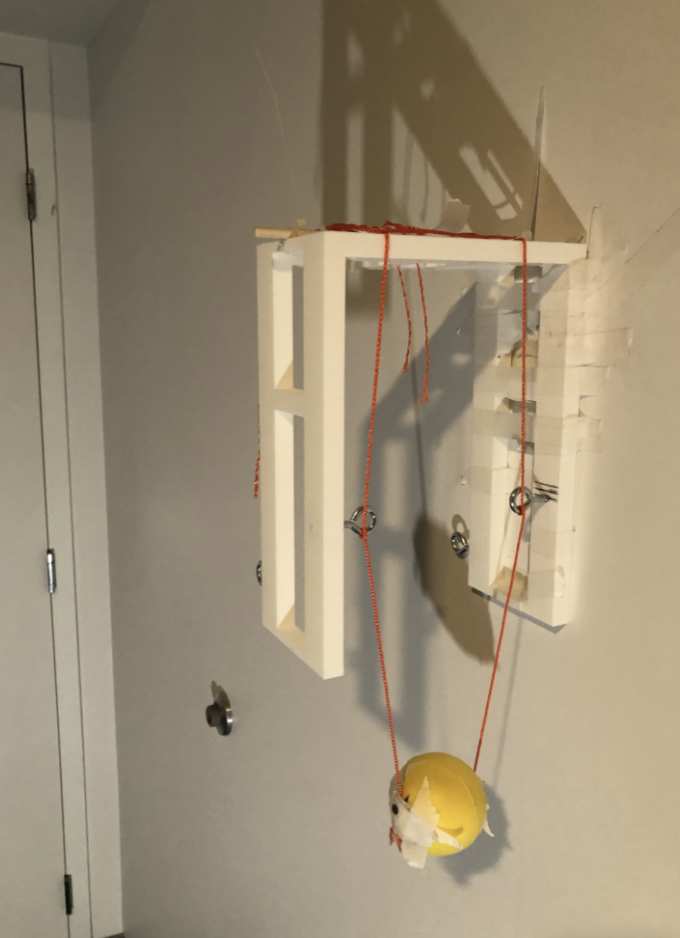
\includegraphics[width=0.4 \textwidth]{images/setup.png}
\label{fig:FallingRock}
\caption{\textcolor{red}{A foam ball is tied to two strings
and each string is held in place by a knot on a
hook. The remaining string is held in tension
with tape at the top of the structure. The
entire structure is severely taped to the wall.}}
\end{centering}
\end{figure}

\textcolor{red}{All videos were taken using an iPad Air camera at 60fps. This was held in place on a
desk with a weight to hold it upright (zero
angle with the horizontal). It was placed at
a distance where the whole apparatus could
be viewed while the pendulum swung.}

\subsection{\textcolor{red}{Period}}

\textcolor{red}{A period was measured by counting the number of frames to complete a cycle. A cycle
begins when the pendulum reaches its lowest
point. The pendulum always passes through
this point, which is also its equilibrium. Since
other points may not be reached as the pendulum continues to oscillate and decay, tracking the period over time is less viable at other
points.}

\textcolor{red}{All presented period values are an average of the
first three periods.}

\textcolor{red}{When comparing the initial angle to the period, 14 measurements were taken, 7 from
positive angles and 7 from negative angles.
The angle of release was measured live to
give a rough estimate and ensure a range
of values was measured. In the post analysis software Tracker, accurate values of the
initial angle were measured with a protractor. Angles measured ranged from -1.36 to
1.42 $\pm$ 0.05 rad with each trial being changed
by 0.17 $\pm$ 0.08 rad.}

\textcolor{red}{The length of the pendulum was fixed for
these trails at L = 43.5 $\pm$ 0.3 cm. All length
measurements were taken using a 30 cm ruler.
The ball was held at the top and bottom and
released by hand.}

\subsection{\textcolor{red}{Q Factor and Angle}}
\textcolor{red}{All Q Factor Measurements were taken
within the range of small angles (maximum
angle of $\theta$ = 26.5 $\pm$ 0.05 rad). All videos were
recorded for at least 60s.}

\textcolor{red}{To measure the angle over time, the Autotracker feature in Tracker was used. The
template was set to Evolve: 40\%, Tether: 5\%,
Automark: 4 and a Step Size: 5. By using
a yellow ball with white tape and a marked
black dot, the reference image of the contrasting black dot was selected. 
This drastically improves the accuracy tracking with
fewer low confidence frames (where the software is unsure if it's tracking the right object). An axis was placed at the pivot point
as a reference point to measure angles.}

\textcolor{red}{Using angle measurements, the amplitude
and the number of oscillations are calculated
from tracker data.}

\textcolor{red}{When comparing pendulum length to Q Factor and period, 8 lengths were considered
ranging from 17.6 to 80.5 $\pm$ 0.5 cm.}

\section{Results and Analysis}
\subsection*{Initial Angle and Period}
\begin{figure}[!h]
    \begin{centering}
    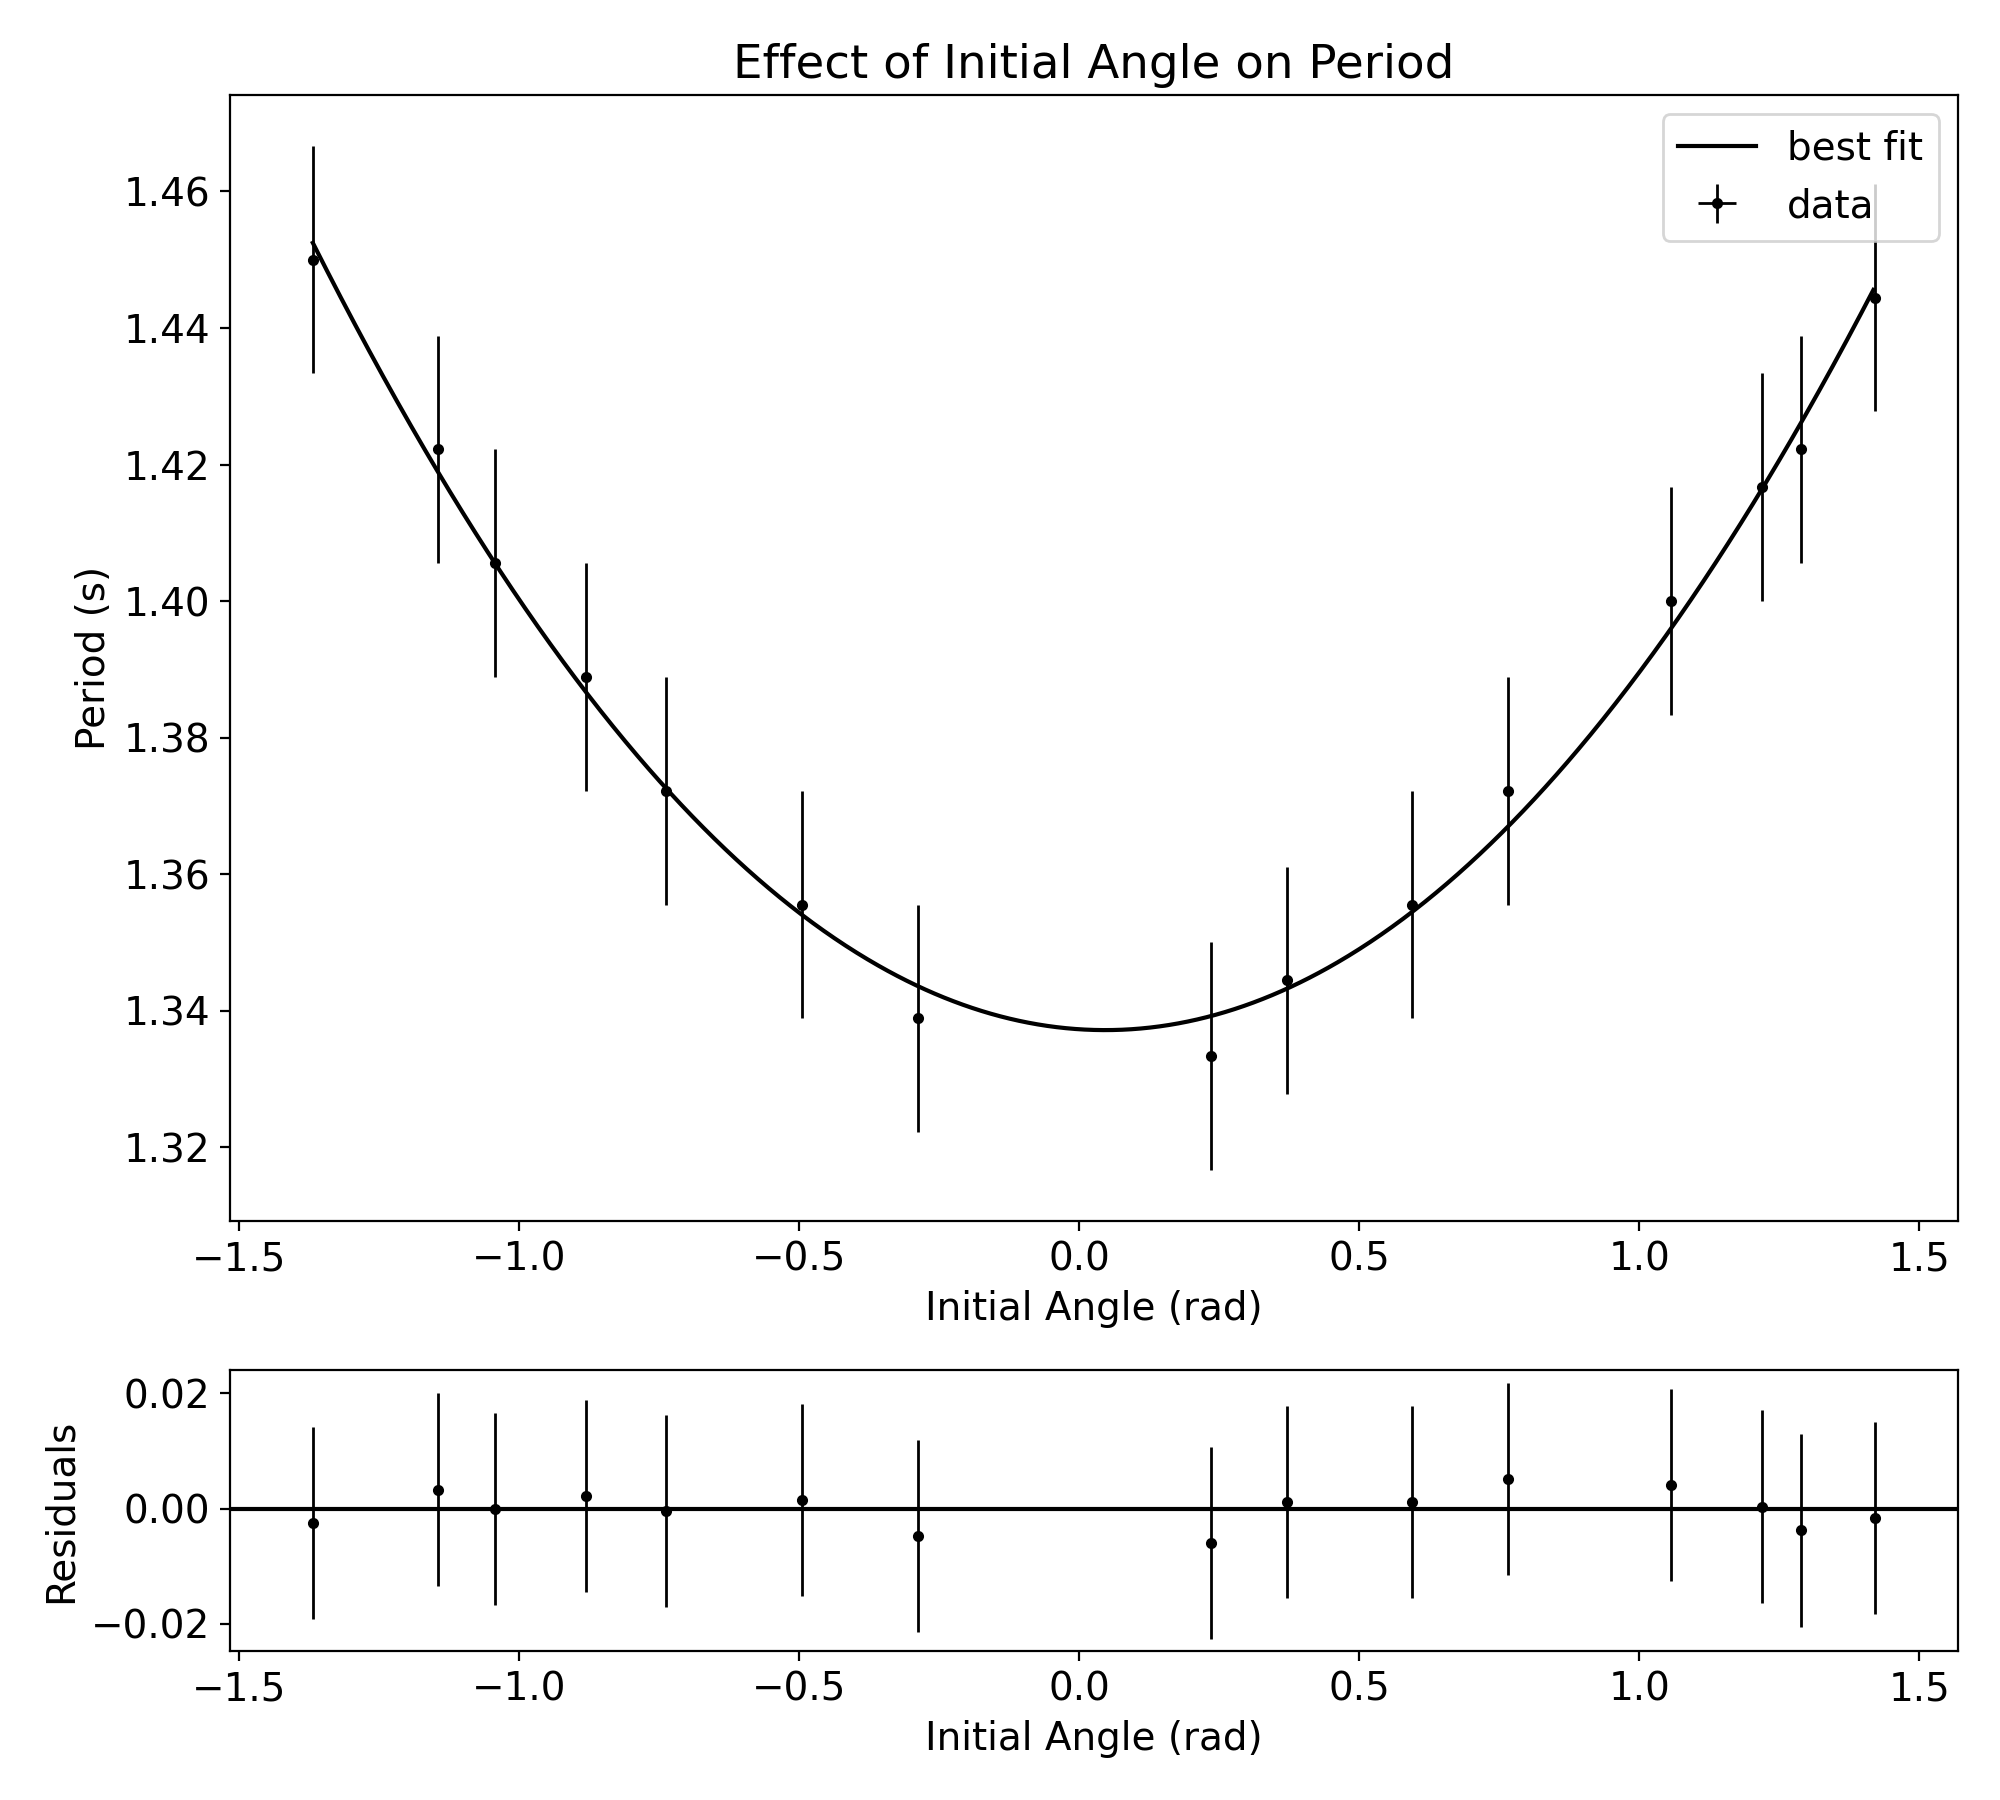
\includegraphics[width=0.5 \textwidth]{images/Effect of Initial Angle on Period.png}
    \label{fig:PeriodAngle}
    \caption{The plot shows how the period
    varies based on the initial angle of release
    for a pendulum of L = 43.5 $\pm$ 0.5 cm. The
    data was fit to the quadratic Equation \ref{Period_Angle}, with parameters 
    $T_0 = 1.337 \pm 0.001 s$,
    $B = -0.003 \pm 0.007 rad^{-1}$,
    $A = 0.043 \pm 0.001 rad^{-2}$.
    A small angle range between $-0.5 \leq \theta
    \leq 0.5 rad$ is present.
    }
    \end{centering}
    \end{figure}

From the fit, the odd term $B$ is found to have a value smaller than its uncertainty,
and therefore is experimentally zero. As a result, the pendulum is symmetric for 
positive and negative angles of release.

The quadratic fit is good since it captures all data points within their uncertainties, and has 
residuals $< 0.02$. The uncertainties of parameters are also low ($\leq 0.001$), giving confidence to the fit.
The small limiting measurement uncertainty of the period $ \pm 0.01s$ and angle $\pm 0.008rad$ support the reasonableness of the results.

Considering all angles, the period varies outside each data's respective uncertainty. 
As the angle of initial release increases, and therefore the amplitude, the period also
increases. Therefore, there is some dependence on amplitude and angle.

However, a small angle range is present: $-0.5 \leq \theta
\leq 0.5 rad$, which lies within
uncertainties for the plotted values in the
angle range. Since the period changes less drastically in this range, through the small angle approximation, releasing the ball within this range allows for period 
values independent of amplitude. Plotting the four points in this range, $A = 0.008 \pm 0.001 rad^{-2}$, which will be considered small since it falls within the period measurement uncertainty of $\pm 0.01s$.
This confirms the absence of the quadratic term in Equation \ref{Period_Angle}, leaving a constant $T = 1.328 \pm 0.002 s$.

\subsection*{Calculating Q Fcator}

\begin{figure}[!h]
\begin{centering}
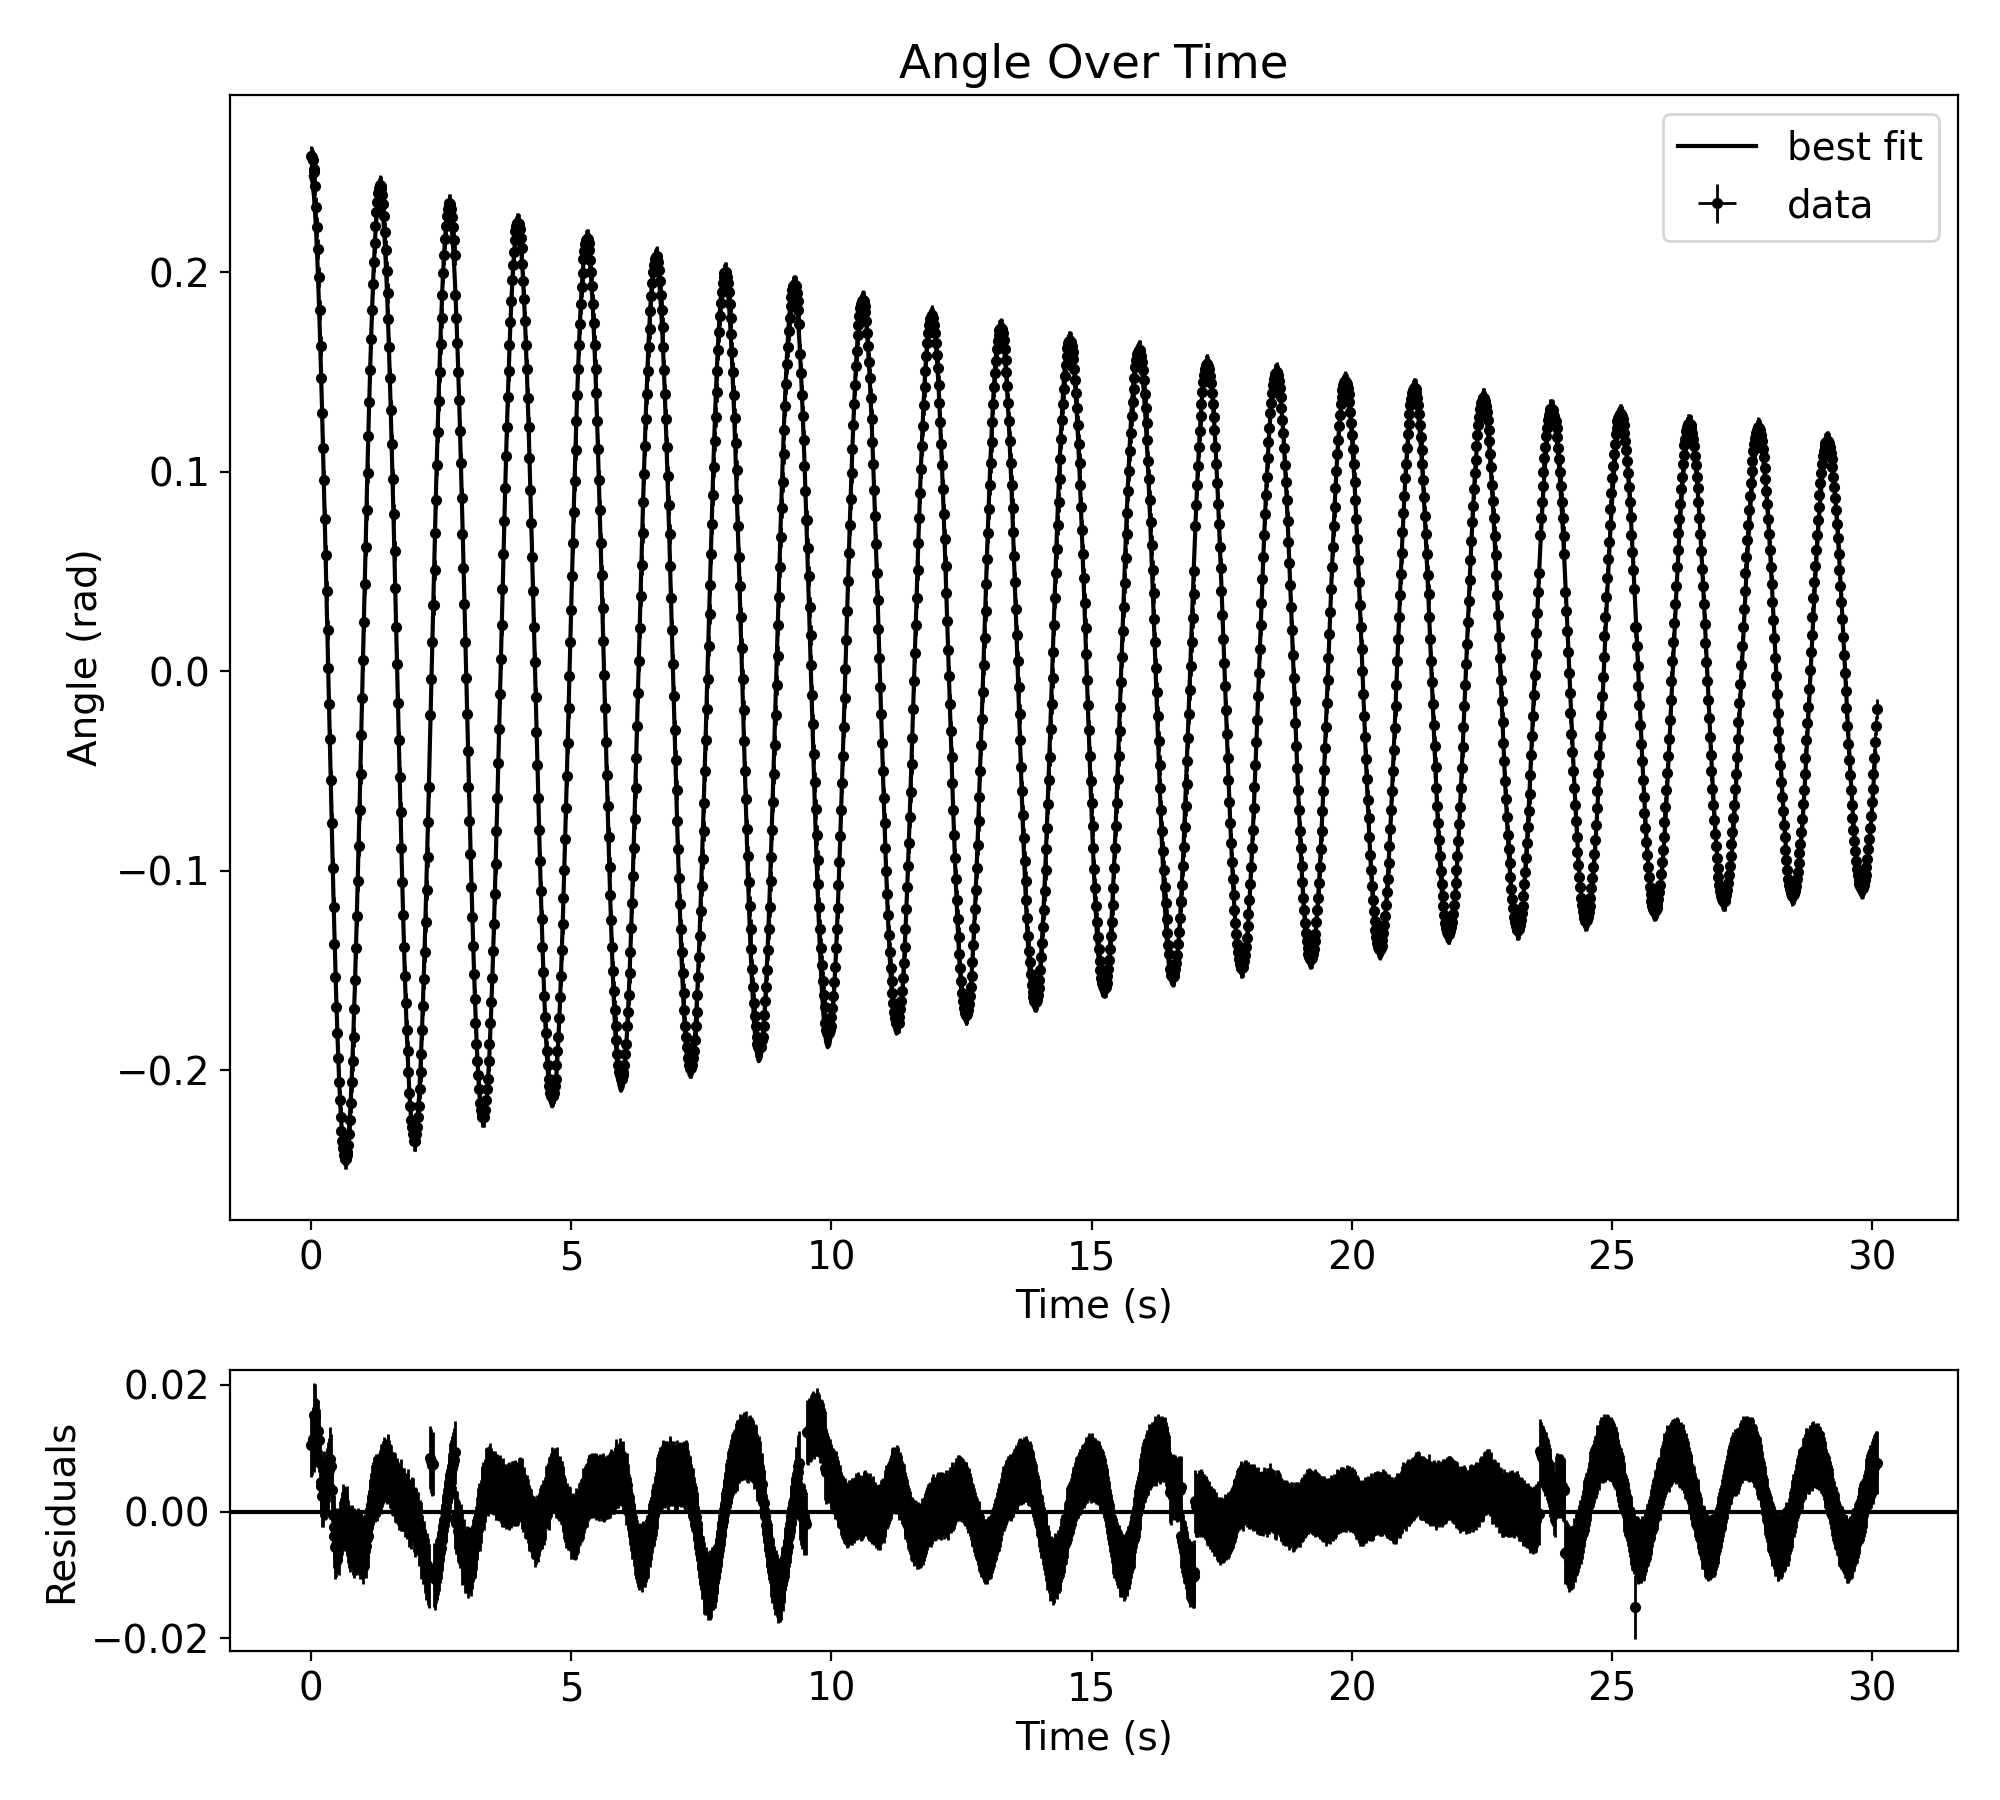
\includegraphics[width=0.5 \textwidth]{images/Angle Over Time.png}
\label{fig:AngleTime}
\caption{The plot shows how the position
of the pendulum, described as an angle from
the vertical, changes over time. The initial angle of release was chosen to be small,
$\theta_0 = 0.235\pm0.005 rad$.  
The best fit parameters for Equation \ref{DampedHarmonic} are
$\theta_0 = 0.2477 \pm 0.0004 rad$, $\tau = 36.3 \pm 0.1 s$, $T =
1.32489 \pm 0.00002s$. A zoomed-in version of the graph with visible error bars
is given in the appendix.
}
\end{centering}
\end{figure}

The damped harmonic model given in Figure \ref{fig:AngleTime} is a good fit since each data point's uncertainties are
captured by the fit and residuals are smaller the 0.02. The uncertainties of fitted parameters are also low ($\leq 0.1$),
giving confidence to the fit. The small limiting measurement uncertainty of the angle ($ \pm 0.008 rad$) support the reasonableness of the results.

From the fitted parameters, Q can be calculated using Equation \ref{Q}. $Q = \pi \frac{36.3\pm0.1}
{1.32489\pm0.00002} = 86.0 \pm 0.1$.

The difference between maximum and minimum angles in each oscillation gives the amplitude. With amplitudes, we can use the
number of oscillations to reach an amplitude
$e^{-\frac{\pi}{k}}\%$ of its initial amplitude. The number of oscillations gives $\frac{Q}{k}$.
The mean Q value from counting oscillation in the k range [2, 8] is $84 \pm 2$. 

The two methods of calculating Q yield the same value within uncertainties and therefore have evidence
they agree with each other

\subsection*{Length and Period}

\begin{figure}[!h]
\begin{centering}
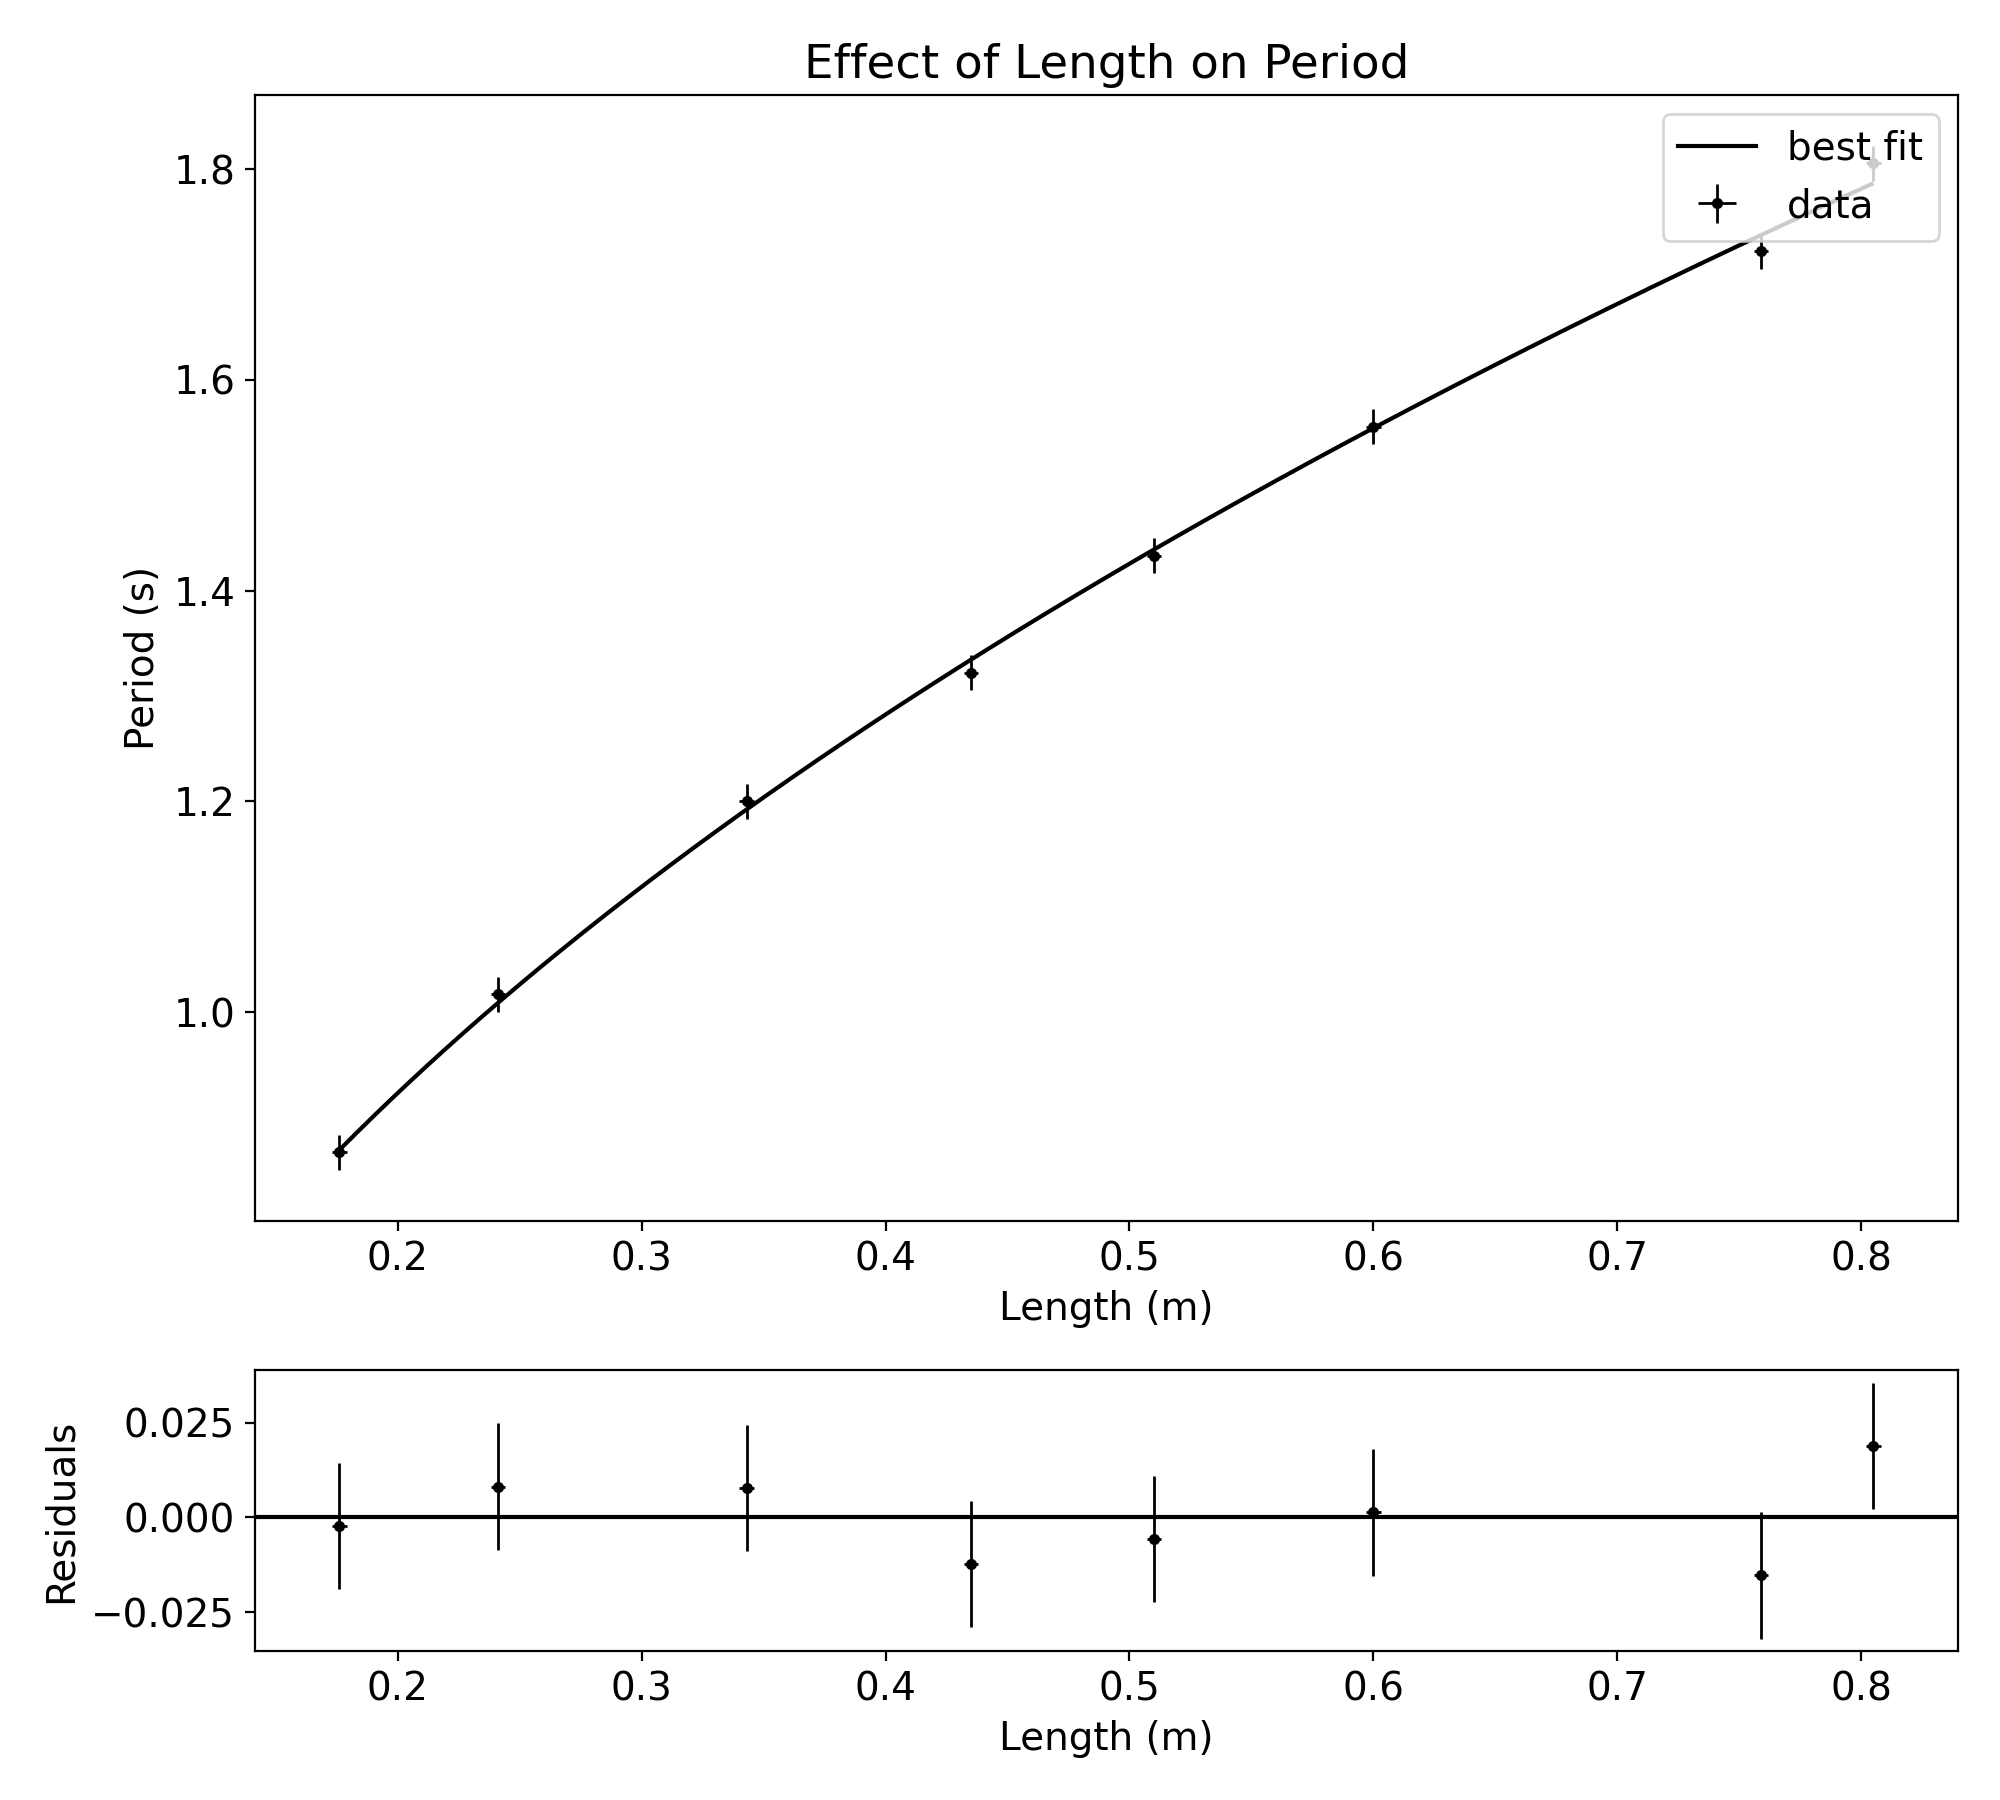
\includegraphics[width=0.5 \textwidth]{images/Effect of Length on Period.png}
\label{fig:LengthPeriod}
\caption{The plot shows how the period
changes based on a pendulum's length. It is
fitted to Equation \ref{Emp_Period}
with parameters $p = 1.98 \pm 0.01 m^{-1}s$ and
$q = 0.474 \pm 0.007$}
\end{centering}
\end{figure}

\begin{figure}[!h]
\begin{centering}
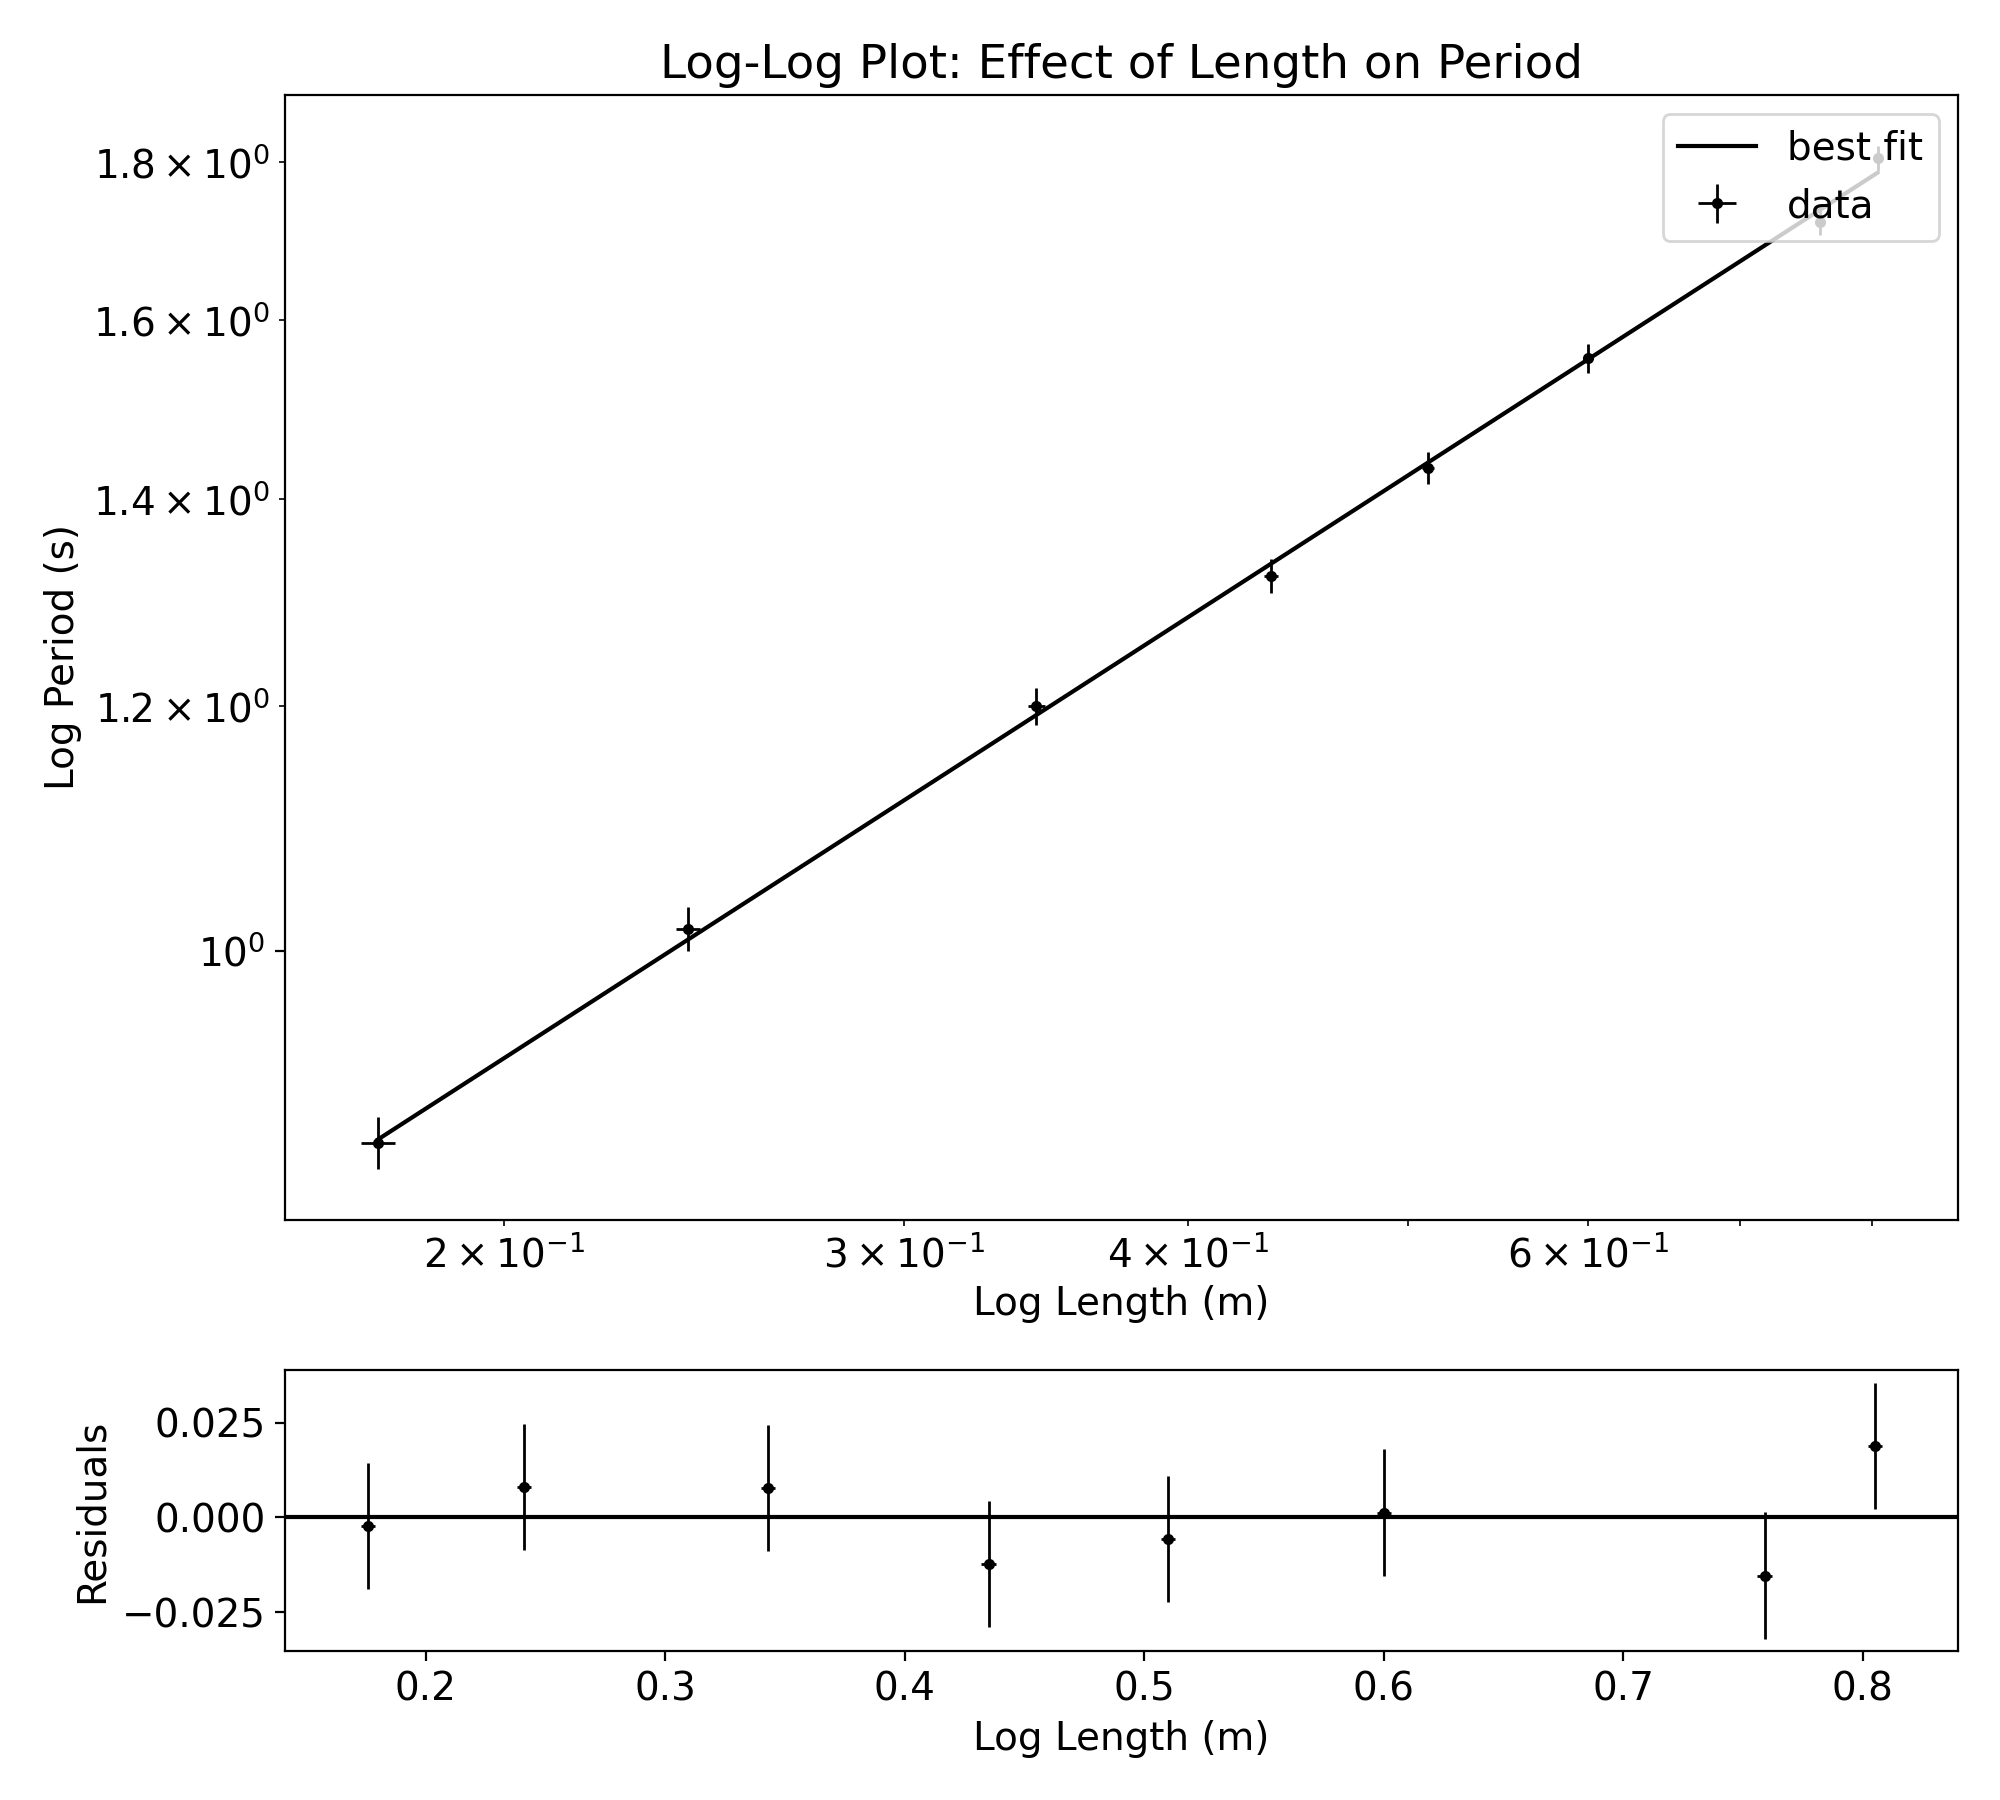
\includegraphics[width=0.5 \textwidth]{images/Log-Log Plot: Effect of Length on Period.png}
\label{fig:LengthPeriodLog}
\caption{Figure 5: The plot displays how the period changes based on a pendulum's length
as a log-log plot fit to a linear function.
The function of y = ax + b has parameters
$a = 1.98 \pm 0.01$ and $b = 0.474 \pm 0.007$.}
\end{centering}
\end{figure}

The power fit captures all data points within their uncertainties with low residuals ($< 0.025$). 
The log-log plot performs even better at fitting the data. The low uncertainties of fitted parameters ($\leq 0.1$)
also give confidence to the fit.
Therefore, the power relationship
between length and period of a pendulum is accurate. The small limiting measurement uncertainty of the length $ \pm 0.003m$ and period $\pm 0.01s$ support the reasonableness of the results.

Given the parameters p and q, and their low range
of fitted uncertainties, the parameters differ from the expected values of p = 2 and
q = 0.5 given by [2]. One reason for this is the fitted uncertainties
are smaller than measurement uncertainties.

\subsection{Q Factor and Length}
Since the uncertainty for calculating Q Factors by Equation \ref{Q} ($\pm 0.1$) is less than
the uncertainty by counting oscillations ($\pm 2$),
Equation \ref{Q} is used.


\begin{figure}[!h]
\begin{centering}
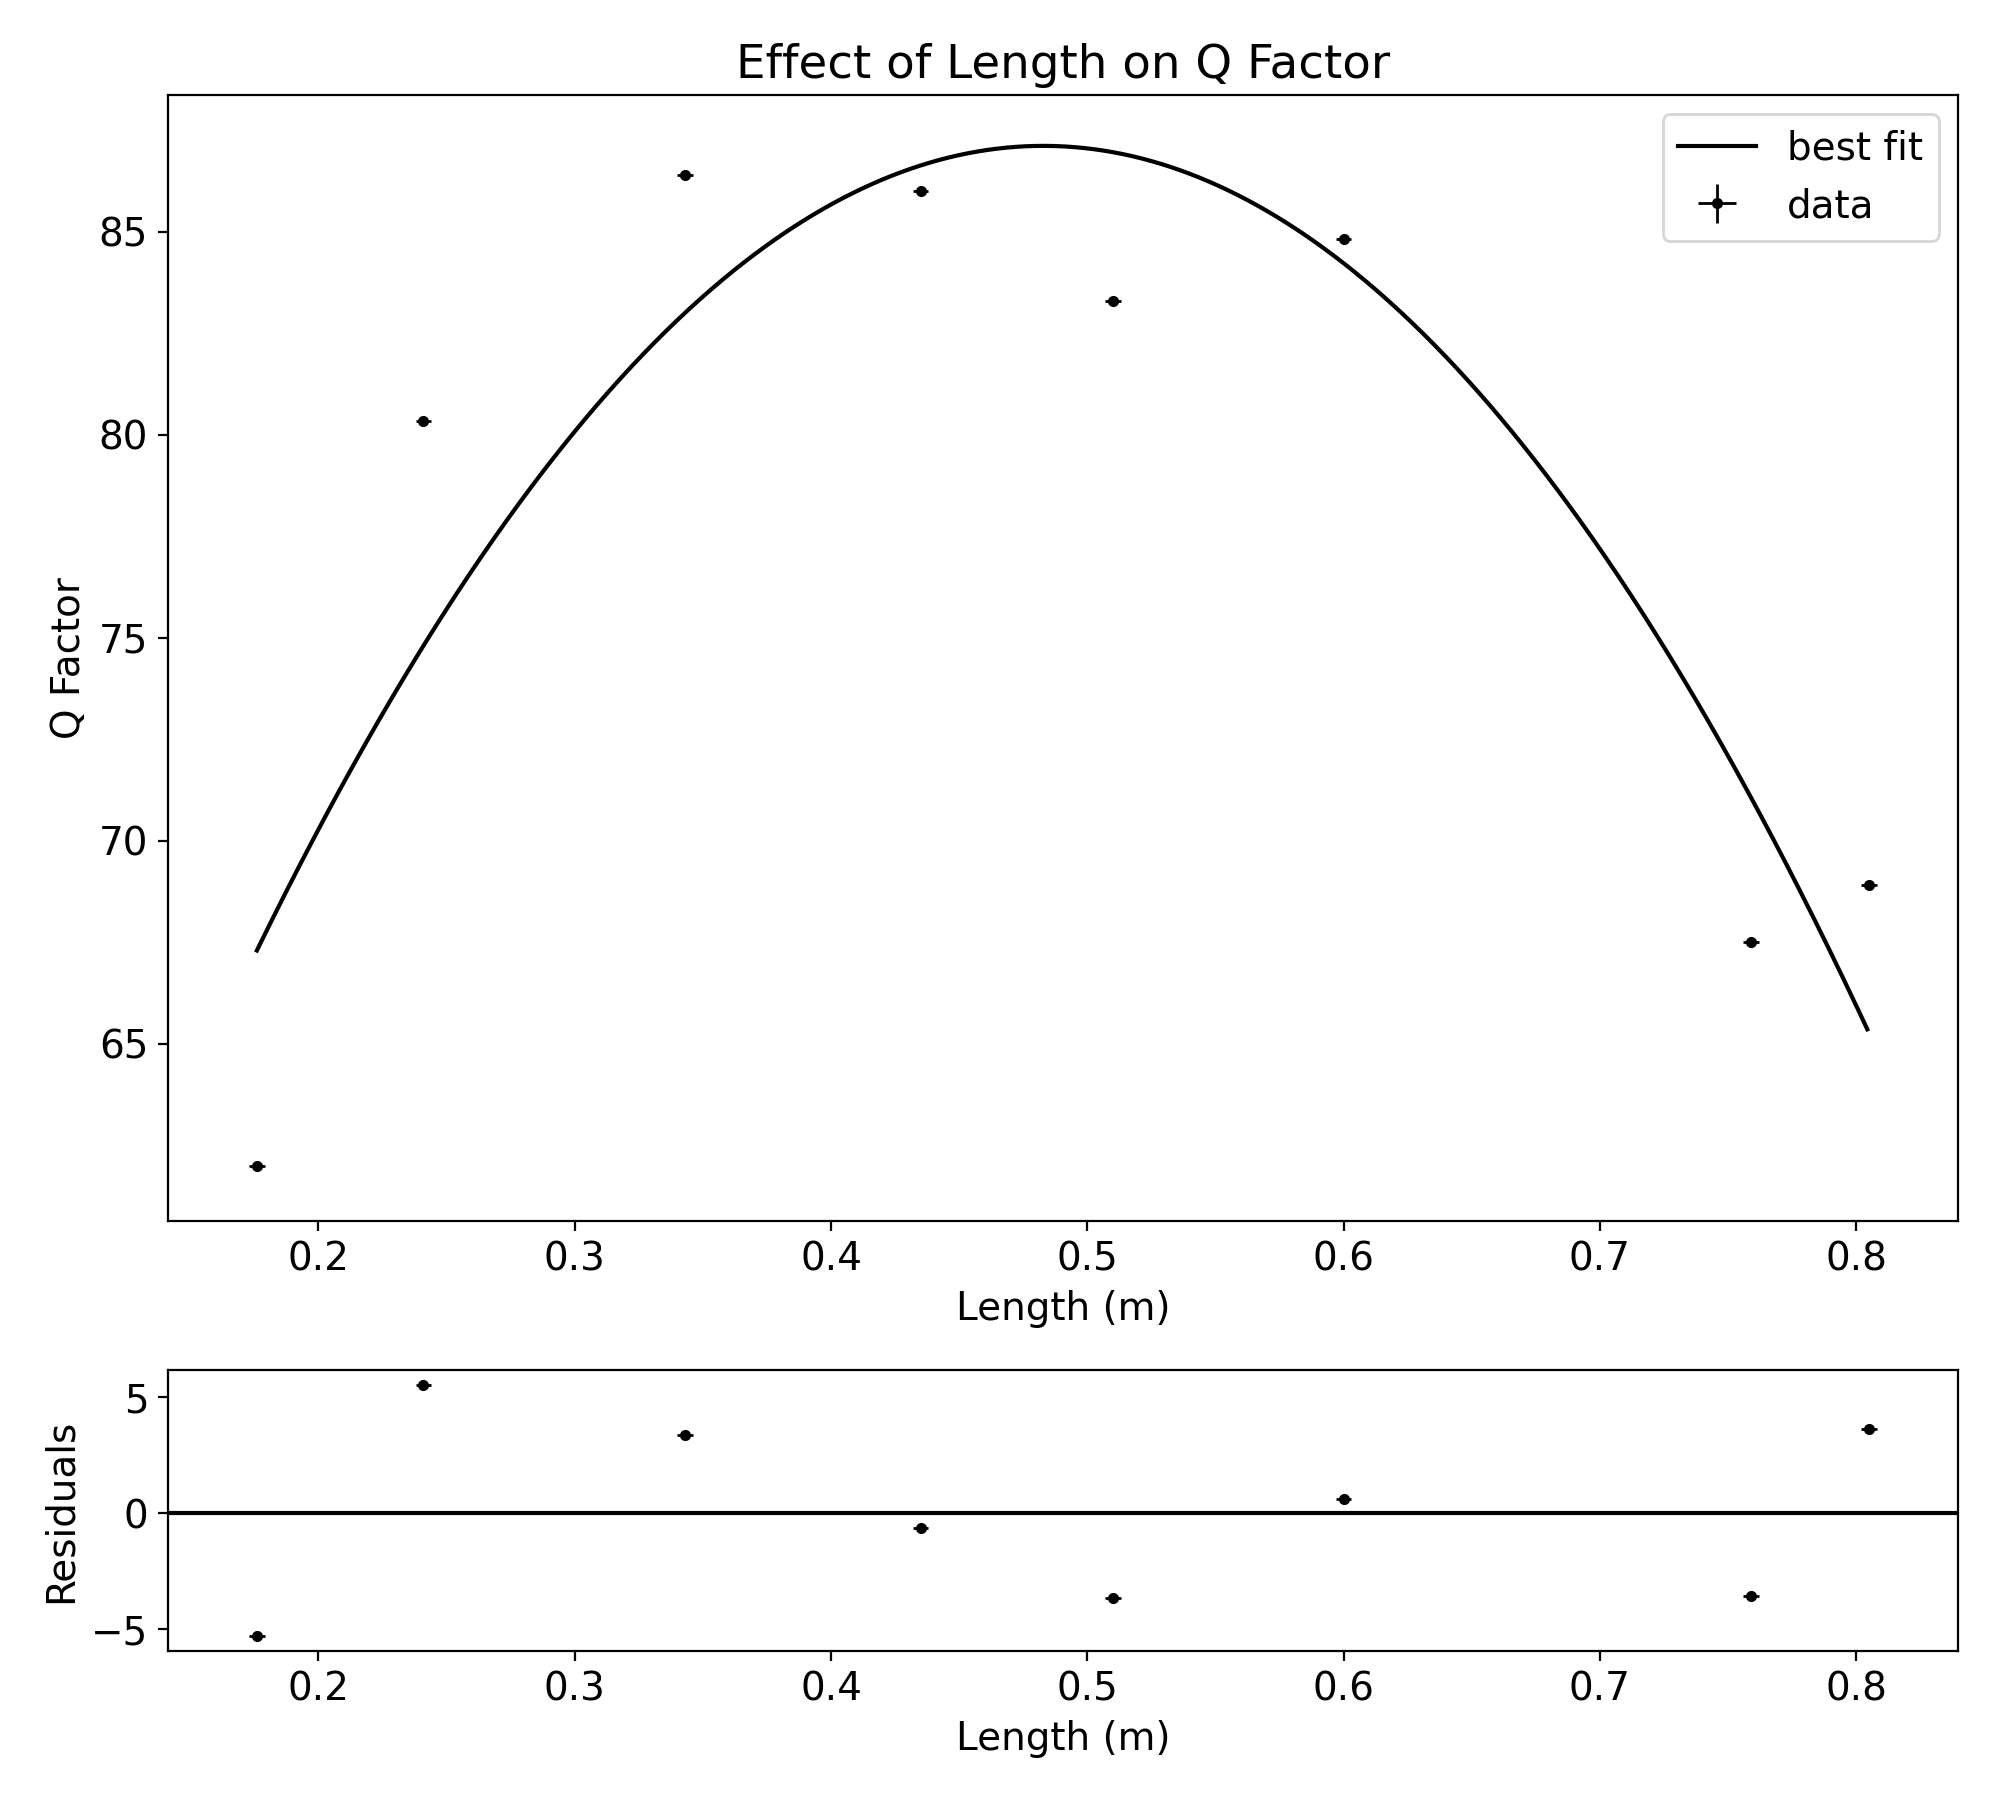
\includegraphics[width=0.5 \textwidth]{images/Effect of Length on Q Factor.png}
\label{fig:QLength}
\caption{The pendulum's Q Factor and
Length are plotted and fitted using a
quadratic function $ax^2 + bx + c$. Where
$a = -210 \pm 42 m^{-2}, b = 200 \pm 43 m^{-1}, c = 30 \pm 9$.
The y uncertainty is given by $\tau$'s fitted uncertainty of $\pm 0.1$.}
\end{centering}
\end{figure}

Given the data points, a quadratic fit most resembles the trend between the Q Factor and length. Despite the similar trend,
the best fit does not capture the values within their y uncertainties ($\pm 0.1$). In addition, the residuals of the plot are high ($> 5$) and outside the uncertainties.
The uncertainty of the coefficients is also high since they are above the measured uncertainties.
This gives low confidence in the fit.

A reason this may have occurred is the slight variation in angle ($\pm 0.05 rad$) for each length measurement. 
This variation may have an effect on $\tau$ unlike how the small approximation was appropriate for the period $T$.


\subsection{Uncertainties}

\textcolor{red}{For Figure \ref{fig:PeriodAngle}, measurement uncertainties exist
for the initial angle and identifying when the
pendulum has reached its lowest point. The
measurement uncertainty due to the precision
of device graduation for the initial angle is
$\pm0.1deg$, which is approximately $\pm0.001rad$.}

\textcolor{red}{There is also uncertainty around where the
protractor is placed in Tracker. Looking at the range in angles for various measurements
at the pivot point to the string gives an uncertainty of $\pm0.008rad$, which is larger than
the previous uncertainty and therefore will be
used. This is calculated by moving the protractor across various points on the vertices
(the pivot point and the ball).}

\textcolor{red}{The period uncertainty is $\pm 1 frame$ or
$\pm 0.01s$ (at 60fps) since empirically, in each
video, the instant at which the pendulum
reaches the bottom lies between two frames.
The time between two frames is $\frac{1}{60}s$. A higher
fps would help reduce this uncertainty.}

\textcolor{red}{Measuring the apparatus uncertainty (how
much results change given the same trial conditions) was difficult due to live measurement
errors and lack of precision. Three independent trials with angles between $0.73\pm0.01rad$
and $0.76 \pm 0.01rad$ yielded the same period values. Therefore, the experimental setup is not the 
largest uncertainty.}

\textcolor{red}{For tracking the angle over time, the angle
measured by Tracker has measurement uncertainties. Since Autotracker is being used,
the point which is tracked on the ball changes
from frame to frame. At 60fps, a random
sample of n = 10 frames is taken and angles
are adjusted to the center. In addition, the
coordinate axis and identification of the ball's
centre itself hold uncertainties in angle measurement. 
In adjusting each of these uncertainties to find the range of angle variation,
the uncertainty given is $\pm0.009rad$. This is
the largest uncertainty. This uncertainty applies to 
Figure \ref{fig:PeriodAngle}.}

\textcolor{red}{Amplitude uncertainty stems from the angle that could be travelled in between frames
when at its highest extremes. It is found that
the ball is in between a maximum of 4 frames
during its highest extremes. This uncertainty
is already small since the ball's angular displacements are smallest at the highest points.
The uncertainty given by the angular velocity
$\omega = 0.002$ over a 4 frame interval at 60fps is
$\pm0.01rad$. However, measurements also differ from tracking uncertainty previously 
mentioned but are smaller than the uncertainty
from potential displacement. The number of
oscillations is a counted value and therefore
has no uncertainty.}

The Q Factor by number of oscillations has a mean error of $\pm 2$ using $\sigma = 6$ and $N = 7$.

\textcolor{red}{Length uncertainties arise from ruler
precision and measurement errors. When
measuring the same pendulum length three
times, the range is found to be $\pm0.3 cm$,
which is greater than the precision uncertainty $\pm0.01 cm$. This is mainly because a
30cm ruler was used, and therefore, the ruler
had to be moved for some measurements. A
measuring tape, rather than a rigid ruler that
spans greater than string length could be used
to reduce error.}

\textcolor{red}{To reduce uncertainties related to the initial angle, clear markings can be placed on
the pivot point and ball to ensure the angle
is measured in the same place, reducing the
amount of angle variation. A more graduated
protractor would also help but likely have significant costs.}

\textcolor{red}{Additional uncertainties involve slightly rotated videos since it has already been 
minimized by post analysis (by slightly rotating
images to become horizontal). Movement in
and out of the video plane has been reduced
by the two-string design.}

\section{Conclusion}
A pendulum's period is dependent on the initial angle release based on the quadratic relationship 
$T = 1.337 \pm 0.001 \times (1 + 0.043 \pm 0.001\theta^2)$. The period is however independent of amplitude in the
small angle range $-0.5 \leq \theta \leq 0.5 rad$ where the squared coefficient $A \approx 0$.

The angle over time is accurately modelled by the damped harmonic oscillator (Equation \ref{DampedHarmonic}).
$\theta(t) = 0.2477 \pm 0.0004 \times e^{\frac{t}{36.3 \pm 0.1}} \times \cos(2\pi \frac{t}{1.32489 \pm 0.00002})$.
Angles are calculated $\pm 0.02 rad$ from their real values and the low coeffecient uncertainties support the model.

This information was used to find a Q Factor. The analytical value using Equation \ref{Q} ($Q = 86.0 \pm 0.1$) and 
mean value ($Q = 84 \pm 2$) from counting the number of oscillations for various decaying amplitude values are found to agree.

The period of a pendulum is found to change based on its length where $L = 1.98 \pm 0.01 L^{0.474 \pm 0.007}$. This
differs slightly from the expected values of $p = 2$ and $q = 0.5$.

The above relationships have high confidence due to uncertainties $\leq 0.1$. The major experimental uncertainty that could be reduced is the angle measurements $\pm 0.008$.
Precision of angle release may also benefit data related to Q Factor and Length, which is found to have no relationship with high uncertainties with fitted parameters.

\appendix
\section*{Appendix}
\subsection*{References}

[1] Brown, D. (2023). Tracker.
\url{https://physlets.org/tracker/}

[2] Wilson, B. (2023). PHY180
Pendulum Project Guidelines.
\url{https://q.utoronto.ca/courses/324650/files/
27269654?module_item_id=4893671}

\begin{figure}[!h]
\begin{centering}
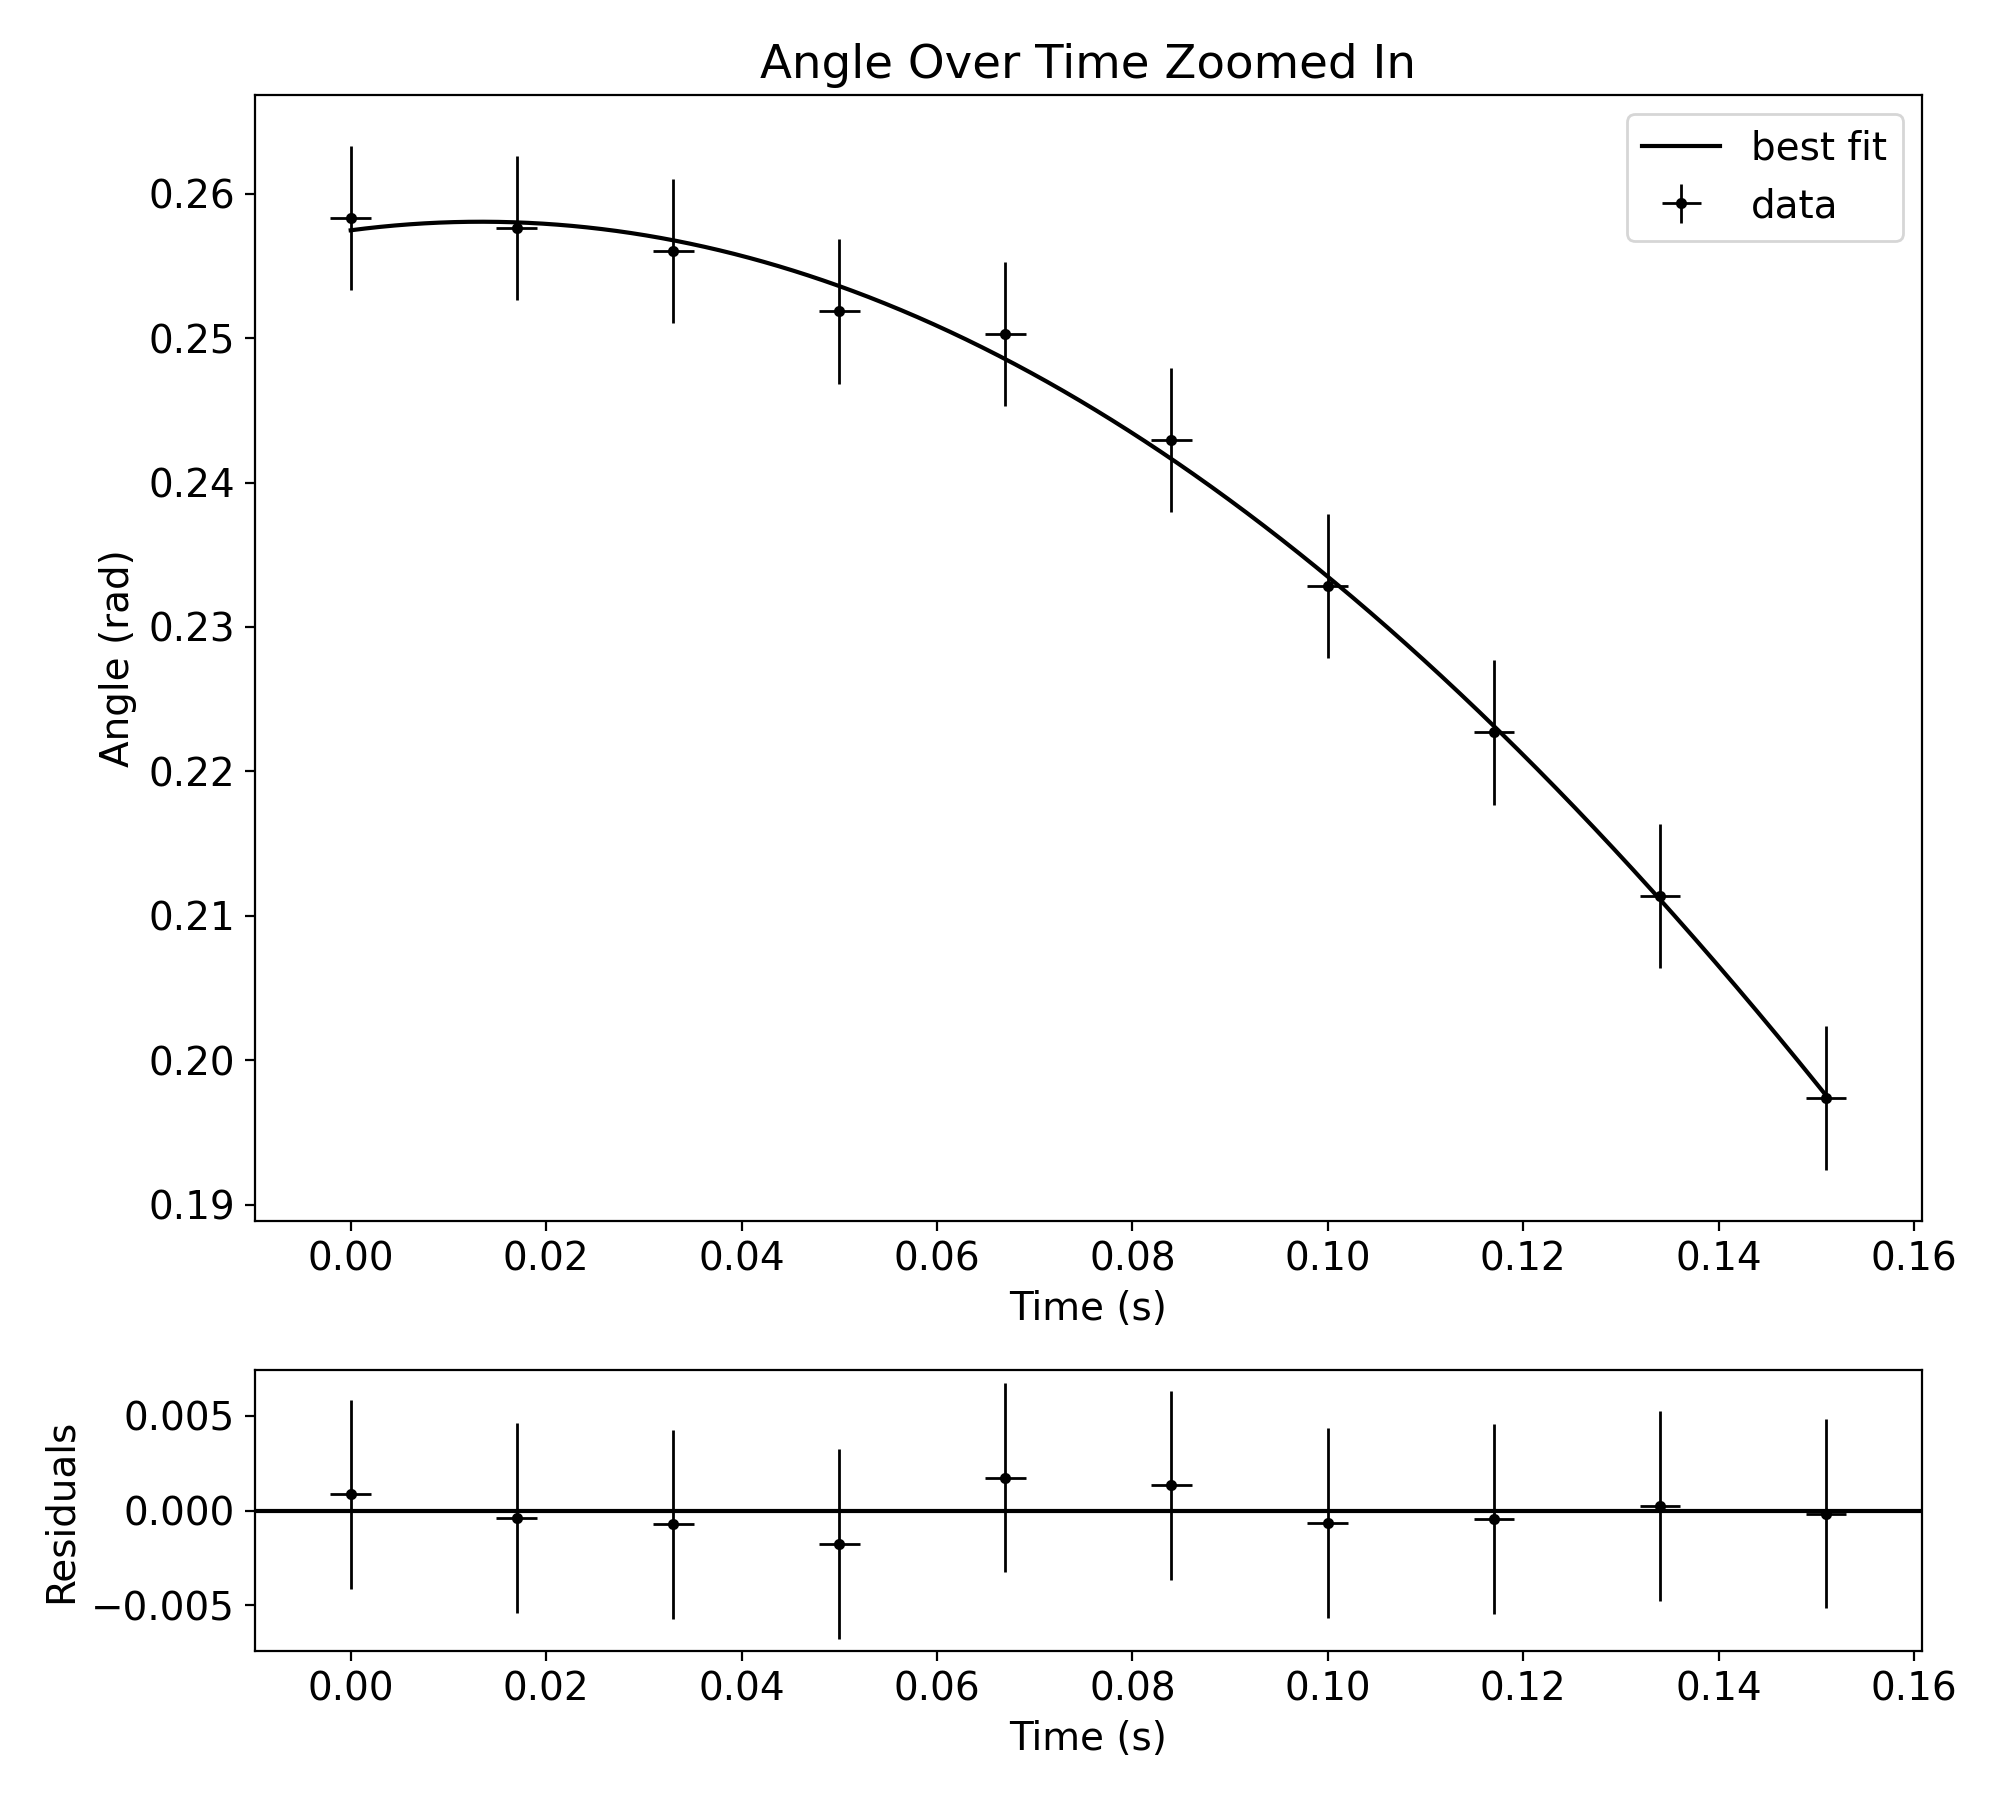
\includegraphics[width=0.5 \textwidth]{images/Angle Over Time Zoomed In.png}
\label{fig:Zoomed}
\caption{\textcolor{red}{A zoomed-in version of Figure 3
with visible error bars. The angle uncertainty is $\pm 0.008rad$}}
\end{centering}
\end{figure}

\begin{figure}[!h]
\begin{centering}
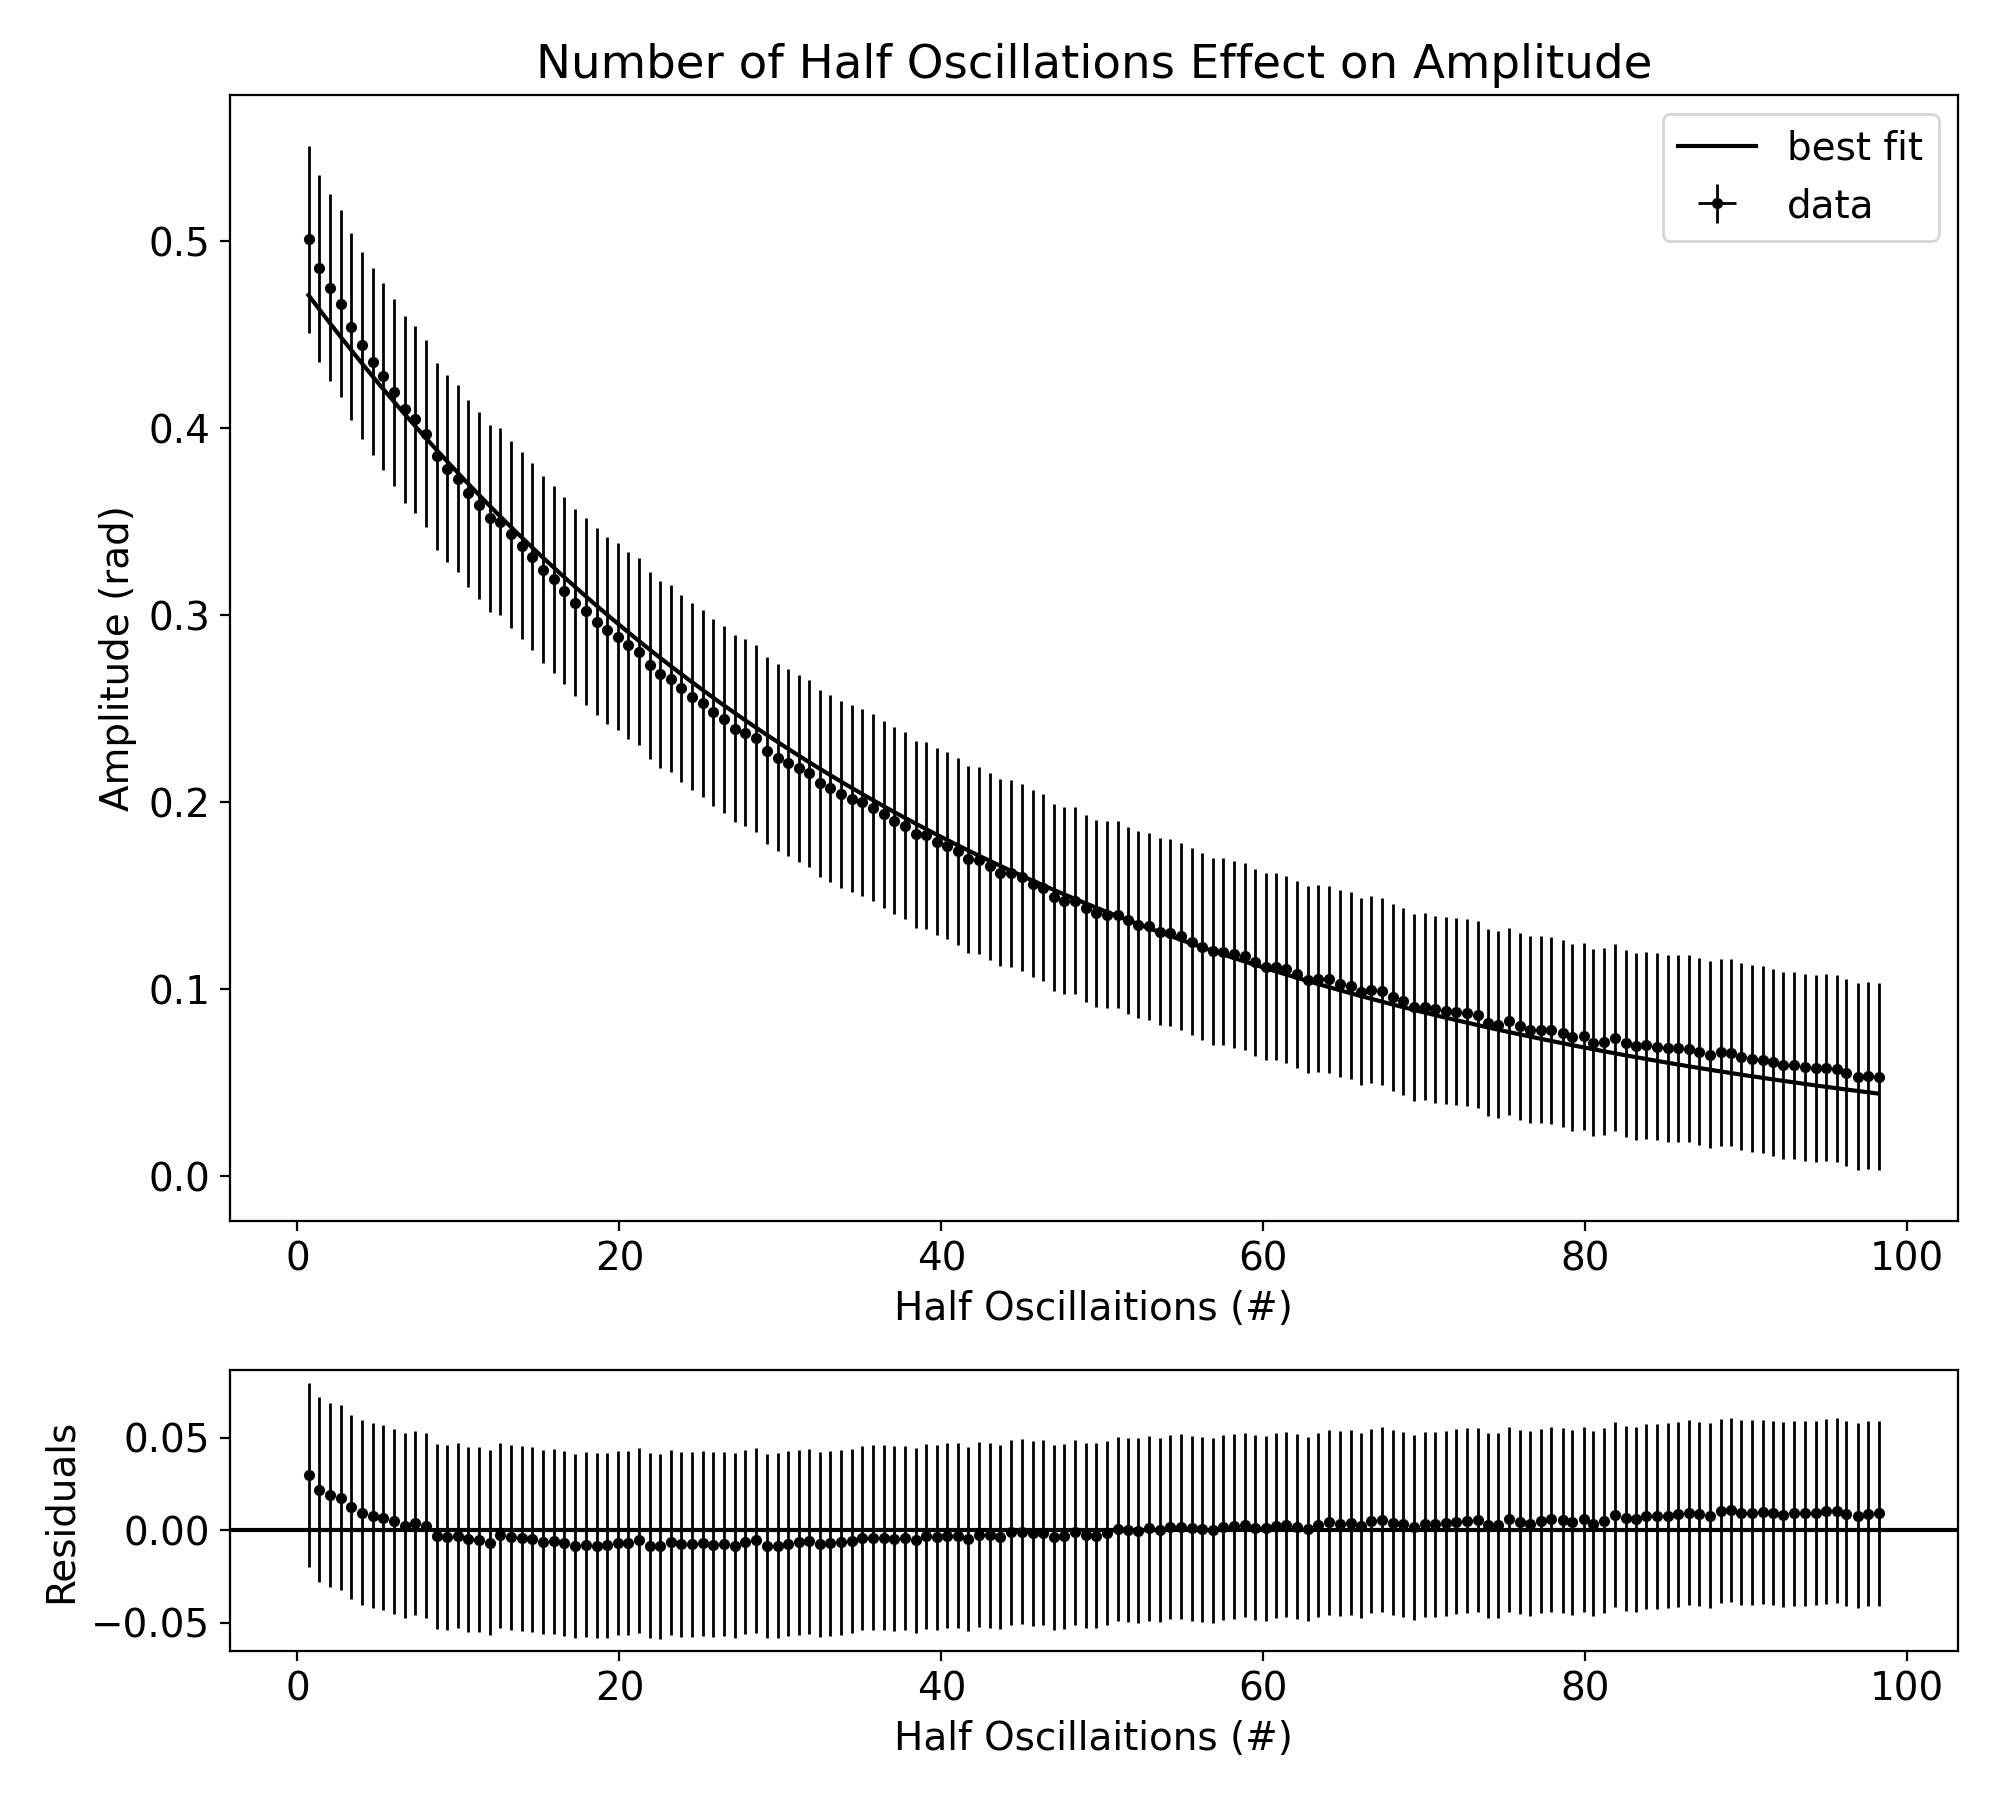
\includegraphics[width=0.5 \textwidth]{images/Number of Half Oscillations Effect on Amplitude.png}
\label{fig:Oscillations}
\caption{\textcolor{red}{This graph confirms how the amplitude decays exponentially as the number
of oscillations increases. The amplitude is
recorded every time a maximum and minimum angle is reached, which is only half an
oscillation.}}
\end{centering}
\end{figure}


\end{document}